\documentclass[runningheads]{llncs}

\usepackage{graphicx}
\usepackage{mathtools}
\usepackage{amsmath}
\usepackage{svg}
\usepackage{xcolor,colortbl}
\usepackage{hyperref}
\renewcommand\UrlFont{\color{blue}\rmfamily}

\begin{document}

\title{Face Verification with Depthwise Separable Convolutions and the Triplet Loss\thanks{Supported by Universidade de São Paulo}}
\titlerunning{Face Verification with Separable Convolutions}

\author{Eduardo S. C. de Souza}

\authorrunning{Carlos de Souza, E. S.}

\institute{Universidade de São Paulo, São Carlos SP, Brazil}

\maketitle

\begin{abstract}
This article explores the use of depthwise separable convolutions and the triplet loss for human face bounding box detection and face verification. The dataset used is the CelebA, consisting of photographic images of celebrities. Experiments executed show that depthwise separable convolutions work considerably well for bounding box detection (1.8\%; 2.01 times faster), but combined with the triplet loss do not perform exceptionally (85\% accuracy; 1.83 times faster).

\keywords{Depthwise Separable Convolutions \and Triplet Loss \and Face Verification}
\end{abstract}



\section{Introduction}

In the field of computer vision, convolutional neural networks have become one of the most popular and effective methods, starting its popularity when AlexNet\cite{NIPS2012_4824} won the ImageNet challenge\cite{ILSVRC15}. It started a currently ongoing trend for such challenges where, in order to achieve better metrics, applicants increase the size, depth, and consequently the computational cost of their models. This results in highly accurate models, but with an unreasonable cost for many applications. As such, it has been a trend in research to take more into consideration the computational cost, and develop ways to optimize CNNs.

In this context, depthwise separable convolutions\cite{sifre2014rigid,howard2017mobilenets} have been widely used. This is due to their considerable reduction in both the number of parameters and computational costs of a CNN, without great loss in accuracy and other such metrics.

\subsection{The Face Verification Problem}

This article aims to apply depthwise separable convolutions to the face verification problem. This problem consists of being able to determine if two images have the face of the same person in them, or different people, without necessarily determining who those people are. It is a variation of the face classification problem, where given a single image, it must be determined to whom the face belongs to in a predetermined set of people.

To achieve this goal, the CNNs will be trained using the Triplet loss function. This is a loss function where, as it decreases, the distances between images belonging to the same class (in this scenario, the same person) decrease, and images belonging to the different classes (in this scenario, different people) increase. As such, the distance between two images is the variable that determines whether or not those two images are of the same person.



\section{Depthwise Separable Convolutions}

\subsection{Number of Weights}

Firstly, the idea of the depthwise separable convolution must be explained in detail. In a regular convolution, the input tensor has rank 3, with the axis being the height, the width, and the number of channels of an input image. Then, each convolutional filter also has rank 3, with the axis being the height and width of the filter and the number of channels of the input image. Each filter will then apply a convolution on the entire input image, each resulting in one output channel of a convolutional layer.

Let $H_{i}$, $W_{i}$, $D_{i}$, $H_{f}$, $W_{f}$, $N_{f}$ be the height of the input image, the width of the input image, the depth (or number of channels) of the input image, the height of the filters, the width of the filters and the number of filters respectively. In a regular convolutional layer, the number of non-bias weights can be expressed by equation \ref{regular_size}.

\begin{equation}
    \label{regular_size}
    N_{f} * H_{f} * W_{f} * D_{i}
\end{equation}

\begin{figure}
    \begin{center}
        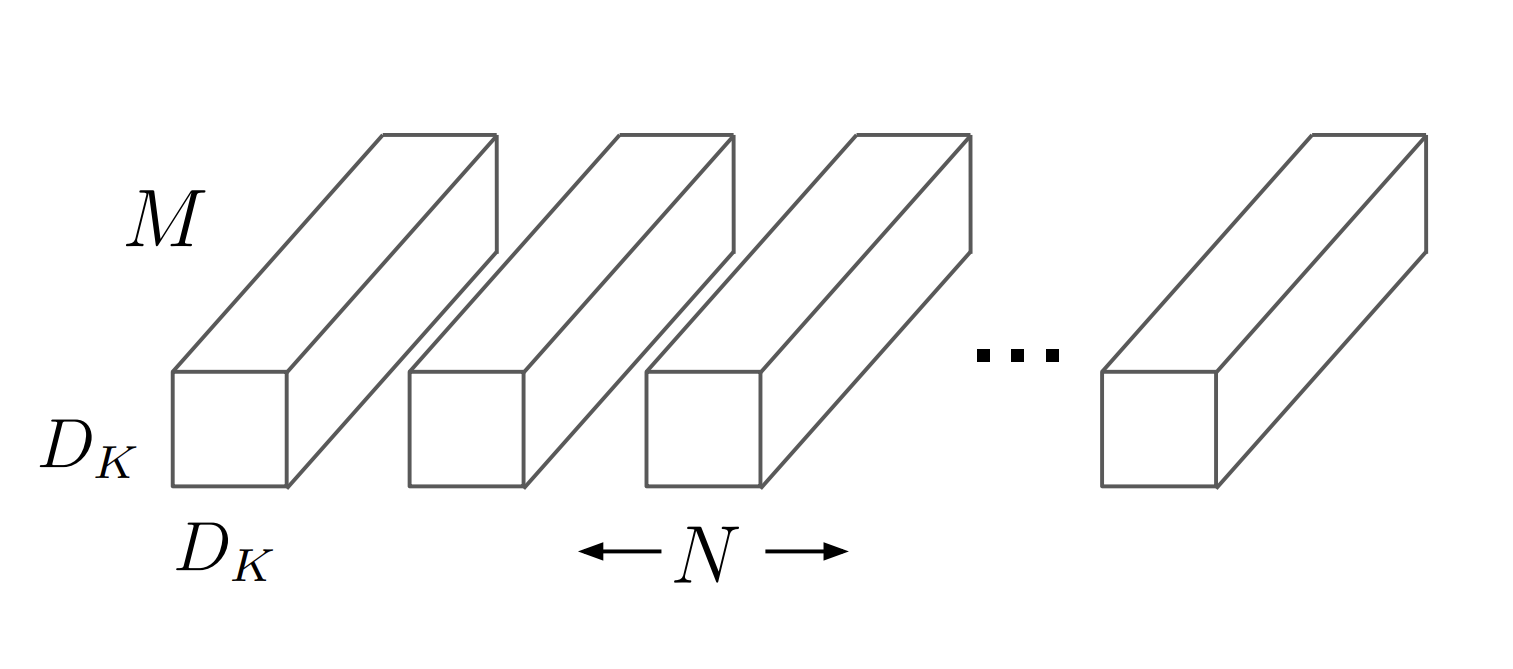
\includegraphics[scale=0.1]{conv_weights_1.png}
        \caption{Shape of a regular convolution's weights}
        \label{conv_weights_1}
    \end{center}
\end{figure}

For a depthwise separable convolution, the input tensor has the same shape. However, the convolution is applied in two steps. The first step consists of executing a convolution on each input channel separately, meaning that both the filters and the images they are applied to will have a depth of 1. Then, the resulting image of each filter will be used as an input channel for the next step. It consists of executing several regular convolutions of size 1x1, known as a pointwise convolution. The resulting image of each pointwise convolution will be one output channel of the depthwise separable convolutional layer.

Image \ref{depthwise_image}, originally from \cite{depthwise_image_towards}, is a good visualization of the way that a depthwise separable convolution is applied.

\begin{figure}
    \begin{center}
        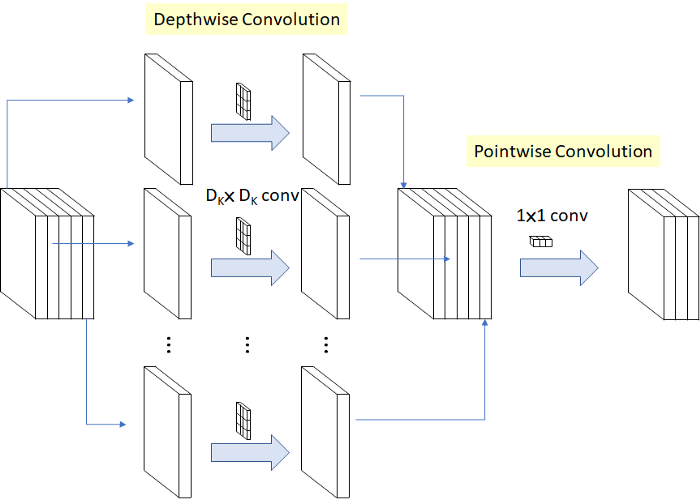
\includegraphics[scale=0.35]{depthwise_sep.png}
        \caption{Both steps of the depthwise separable convolution}
        \label{depthwise_image}
    \end{center}
\end{figure}

The number of non-bias weights for a depthwise separable convolution can be expressed by equation \ref{separable_size}. The first element of the sum refers to the weights on the first step of the process, and the second element to the second step.

\begin{equation}
    \label{separable_size}
    D_{i} * H_{f} * W_{f} + D_{i} * N_{f} 
\end{equation}

\begin{figure}
    \begin{center}
        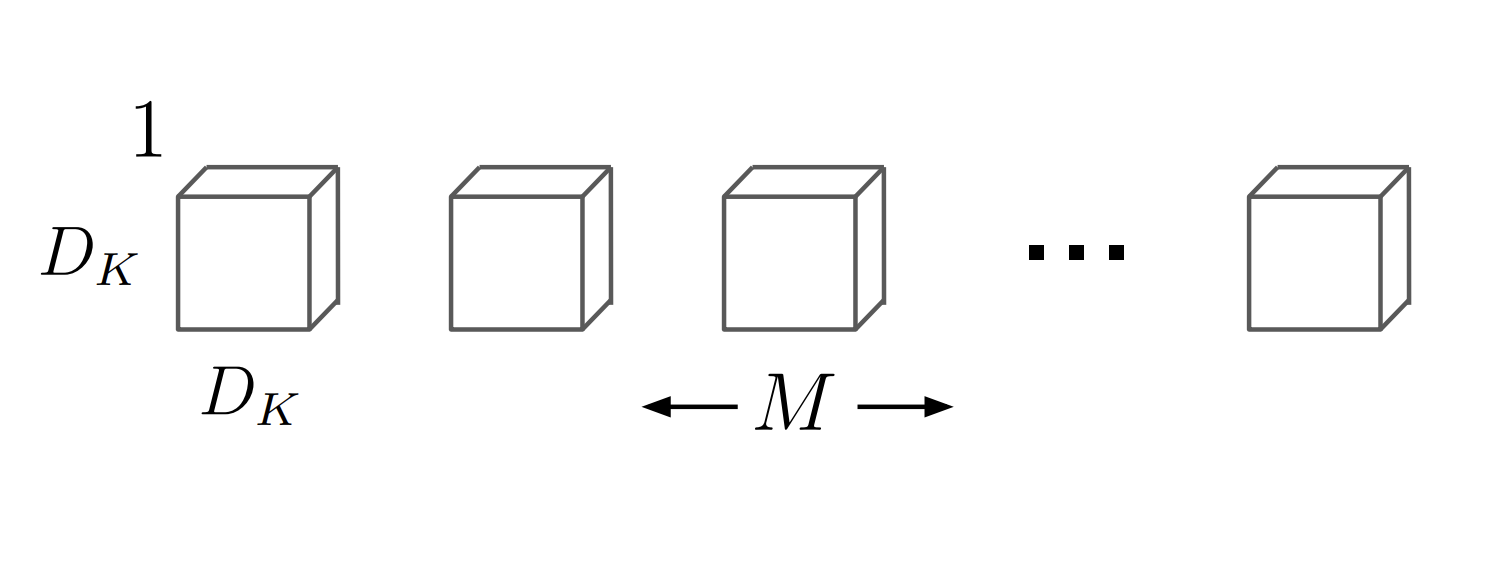
\includegraphics[scale=0.1]{conv_weights_2.png}
        \caption{Shape of a depthwise separable convolution's first step's weights}
        \label{conv_weights_2}
    \end{center}
\end{figure}

\begin{figure}
    \begin{center}
        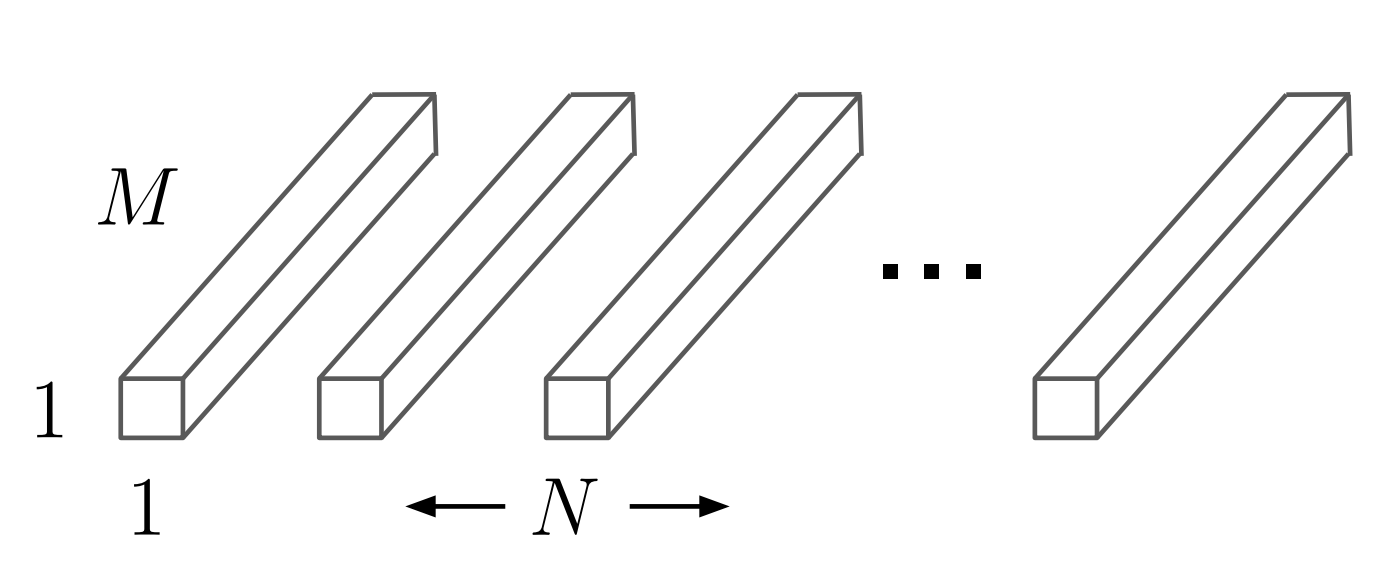
\includegraphics[scale=0.1]{conv_weights_3.png}
        \caption{Shape of a depthwise separable convolution's second step's weights}
        \label{conv_weights_3}
    \end{center}
\end{figure}

Therefore, the ratio between the number of weights can be expressed by equation \ref{weights_ratio}, showing a considerable reduction in the number of weights.

\begin{align}
    \label{weights_ratio}
    \begin{aligned}
        & \frac{ D_{i} * H_{f} * W_{f} + D_{i} * N_{f} }{ N_{f} * H_{f} * W_{f} * D_{i} }
        = \frac{ D_{i} * (H_{f} * W_{f} + N_{f}) }{ N_{f} * H_{f} * W_{f} * D_{i} } = \\ \\
        & \frac{ H_{f} * W_{f} + N_{f} }{ H_{f} * W_{f} * N_{f} }
        = \frac{ 1 }{ N_{f} } + \frac{ 1 }{ H_{f} * W_{f} }
    \end{aligned}
\end{align}

Images \ref{conv_weights_1}, \ref{conv_weights_2} and \ref{conv_weights_3}, originally from \cite{howard2017mobilenets}, are a good visualization of the weights in each type of convolution.

\subsection{Number of Operations}

Although the number of parameters is certainly important, in many scenarios the number of operations is considerably more so. Assuming a stride of 1, and sufficient padding so that the output has the same height and width as the input, the number of sums and multiplications executed by a regular convolution can be expressed by equation \ref{regular_cost}.

\begin{equation}
    \label{regular_cost}
    N_{f} * H_{i} * W_{i} * H_{f} * W_{f} * D_{i}
\end{equation}

With the same assumptions, the number of operations executed by a depthwise separable convolution can be expressed by equation \ref{separable_cost}. The first element of the sum refers to the operations on the first step of the process, and the second element to the second step.

\begin{equation}
    \label{separable_cost}
    D_{i} * H_{i} * W_{i} * H_{f} * W_{f} + N_{f} * H_{i} * W_{i} * D_{i}
\end{equation}

And the ratio between the number of operations can be expressed by equation \ref{cost_ratio}, showing a considerable reduction in the computational cost.

\begin{align}
    \label{cost_ratio}
    \begin{aligned}
        & \frac{ D_{i} * H_{i} * W_{i} * H_{f} * W_{f} + N_{f} * H_{i} * W_{i} * D_{i} }{ N_{f} * H_{i} * W_{i} * H_{f} * W_{f} * D_{i} } = \\ \\
        & \frac{ D_{i} * (H_{i} * W_{i} * H_{f} * W_{f} + N_{f} * H_{i} * W_{i}) }{ N_{f} * H_{i} * W_{i} * H_{f} * W_{f} * D_{i} } = \\ \\
        & \frac{ H_{i} * W_{i} * H_{f} * W_{f} + N_{f} * H_{i} * W_{i} }{ N_{f} * H_{i} * W_{i} * H_{f} * W_{f} } = \\ \\
        & \frac{ H_{i} * W_{i} * H_{f} * W_{f} }{ N_{f} * H_{i} * W_{i} * H_{f} * W_{f} } + \frac{ N_{f} * H_{i} * W_{i} }{ N_{f} * H_{i} * W_{i} * H_{f} * W_{f} } = \\ \\
        & \frac{ 1 }{ N_{f} } + \frac{ 1 }{ H_{f} * W_{f} }
    \end{aligned}
\end{align}



\section{Triplet Loss}

The triplet loss\cite{schroff2015facenet} is a loss function that aims to move feature vectors belonging to the same class closer to each other. It does this by a fairly simpĺe method, which is by explicitly minimizing the distance between samples of the same class, and maximizing the distance between samples of different classes. Its equation is the number \ref{triplet_function}.

\begin{equation}
    \label{triplet_function}
    l(A, P, N) = max(0, d(f(A), f(P)) - d(f(A), f(N)) + \alpha)
\end{equation}

Where $A$ is the anchor sample, $P$ is the positive sample, which means it should be clustered with $A$ (belongs to the same class), and $N$ is the negative sample, which means it should be moved away from $A$ (belongs to a different class). $f$ is the function that generates a feature vector from an input, such as a CNN. $d$ is a function that calculates the distance between 2 vectors, commonly being the euclidean distance or the euclidean distance squared. $\alpha$ is a constant, which serves as a margin, or a minimum difference, between the positive and negative examples. It exists so that in cases where the negative distance is just slightly greater than the positive the loss doesn't become zero. The maximum with 0 serves as a lower limit for the function.

\begin{figure}
    \begin{center}
        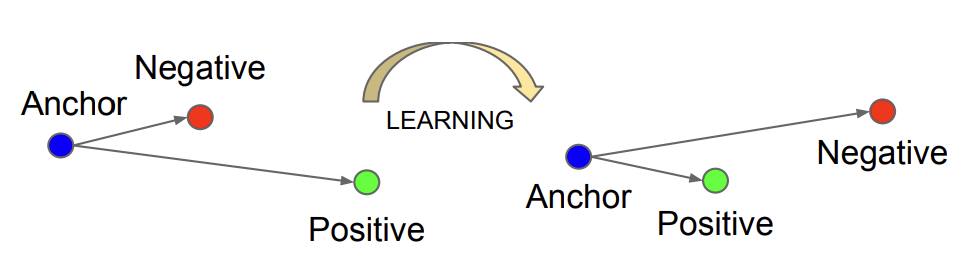
\includegraphics[scale=0.25]{triplet_graph.png}
        \caption{Effects of training with the triplet loss}
        \label{triplet_graph}
    \end{center}
\end{figure}

The triplet loss decreases either when the distance between the anchor and the positive example decrease, or when the distance between the anchor and the negative example increase. As such, as its value reduces through the training process, the feature vectors start to become clustered based on their classes. The effects of triplet loss reduction is shown in image \ref{triplet_graph}, originally from \cite{schroff2015facenet}.

In the context of the face verification problem, the anchor would be an image of someone, the positive sample would be a different image of the same person, and the negative sample a tertiary image of a different person. It is expected then, that a feature extractor with a low triplet loss is capable of generating highly representative feature vectors of human faces.

\subsection{Types of Triplets}

Triplets can be separated into three groups: easy, hard, and semi-hard.

\begin{itemize}
    \item The easy triplets occur when the distance from the anchor to the negative sample is already greater than the distance from the anchor to the positive sample plus the $\alpha$ margin.
    
    \item The hard triplets occur when the distance to the negative sample is smaller than the one to the positive sample.
    
    \item The semi-hard triplets occur when the distance to the negative sample is greater than the one to the positive sample, but not greater than the distance to the positive sample plus the $\alpha$ margin. 
\end{itemize}

This distinction is easily visualized on image \ref{triplet_diff_img}, originally from \cite{triplet_diffs}.

\begin{figure}
    \begin{center}
        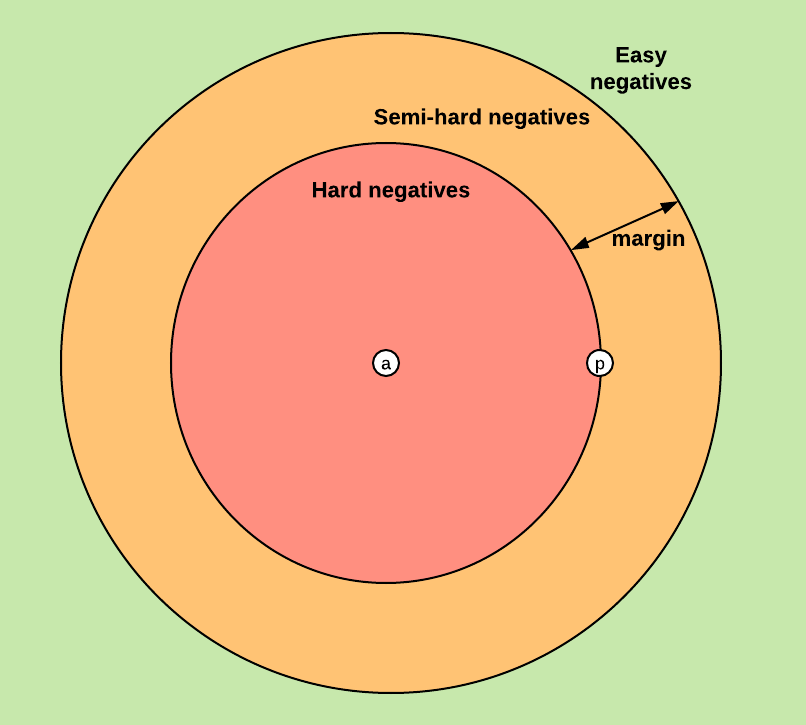
\includegraphics[scale=0.6]{triplet_diff.png}
        \caption{Differences in types of triplets}
        \label{triplet_diff_img}
    \end{center}
\end{figure}



\section{Experiments}

The main goal of this article is to explore the use of both the previously mentioned techniques on the face verification problem. The problem is broken down into two steps.

\begin{enumerate}
  \item \textbf{Bounding Box Detection and Segmentation:} The first step is to create a model capable of detecting the bounding box of someone's face on an image. It is limited to a single face per image.
  \item \textbf{Verification Through Feature Vector Distance:} The next step is to create a model capable of generating feature vectors for the segmented faces. The distance between 2 extracted feature vectors is then used to differentiate between the same person and different people.
\end{enumerate}

\subsection{Dataset and Tools Used}

For both steps the CelebA\cite{liu2015faceattributes} dataset is used, since it has all the annotation needed, and is extremely large and varied. The version of the dataset used is the in-the-wild one, since it represents a real-world scenario. For the verification step, the images are cropped using the ground-truth bounding boxes, so as not to propagate errors from the segmentation model. Also, only images of individuals with more than 5 images of them in the dataset were used. The implementation used the TensorFlow\cite{tensorflow2015-whitepaper} platform.

\subsection{Bounding Box Detection and Segmentation}

This problem is modeled as a regression problem, where the input is the image, and the expected output is the location of each of the 4 edges of the bounding box. The positions of the edges are normalized by the image shape so that the regression is always in the $\left[0, 1\right]$ interval.

The models used for this step are all CNNs, separated into two groups; one that uses regular convolutions, and one that uses depthwise separable convolutions. Each group is a grid search of models architectures, varying the input image size, the depth, the number of convolutional filters, and the size of the dense layers. This resulted in 54 different models for each group.

The images were in the RGB color space, all input pixels where divided by 255 so they fall in the $\left[0, 1\right]$ interval, and the image resized to the CNNs input shape using the bi-linear interpolation. All data used 32-bit floating-point variables. 

All models were trained using the Adamax optimizer, for a maximum of 1000 epochs, with the possibility of early stopping. Each epoch consisted of 200 batches of 32 samples, and after each epoch 50 batches of 32 samples were used to extract validation metrics. The mean squared error was used as the loss function. After training was over, the weights with the best metrics during training are restored and stored, and the model with those weights is evaluated on 2000 batches of 32 images.

\begin{figure}
    \includesvg[width=\textwidth]{regular_all_loss.svg}
    \caption{Validation loss during training for all models using regular convolutions}
    \label{regular_all_loss}
\end{figure}

\begin{figure}
    \includesvg[width=\textwidth]{regular_all_iou.svg}
    \caption{Validation IoU during training for all models using regular convolutions}
    \label{regular_all_iou}
\end{figure}

\begin{figure}
    \includesvg[width=\textwidth]{regular_top_loss.svg}
    \caption{Validation loss during training for the top 5 models using regular convolutions}
    \label{regular_top_loss}
\end{figure}

\begin{figure}
    \includesvg[width=\textwidth]{regular_top_iou.svg}
    \caption{Validation IoU during training for the top 5 models models using regular convolutions}
    \label{regular_top_iou}
\end{figure}

\begin{figure}
    \includesvg[width=\textwidth]{separable_all_loss.svg}
    \caption{Validation loss during training for all models using depthwise separable convolutions}
    \label{separable_all_loss}
\end{figure}

\begin{figure}
    \includesvg[width=\textwidth]{separable_all_iou.svg}
    \caption{Validation IoU during training for all models using depthwise separable convolutions}
    \label{separable_all_iou}
\end{figure}

\begin{figure}
    \includesvg[width=\textwidth]{separable_top_loss.svg}
    \caption{Validation loss during training for the top 5 models models using depthwise separable convolutions}
    \label{separable_top_loss}
\end{figure}

\begin{figure}
    \includesvg[width=\textwidth]{separable_top_iou.svg}
    \caption{Validation IoU during training for the top 5 models models using depthwise separable convolutions}
    \label{separable_top_iou}
\end{figure}

The models using depthwise separable convolutions generally took longer to train, as is more easily noticeable when comparing images \ref{regular_top_loss} and \ref{separable_top_loss}. Also, they only had slightly worse metrics, shown in images \ref{regular_top_iou} and \ref{separable_top_iou}.

One notable problem with depthwise separable convolutions is the possibility of the loss not decreasing due to a local minimum, as seen in image \ref{separable_all_loss}. During training, very similar models, or sometimes the same model with different initial weights, will have different behaviors regarding non-convergence. This points to the loss getting stuck on a local minimum being the cause.

This occurs in only one instance in all regular convolution models (kept out of the graph due to being in a very different range), but in many cases in the separable models, especially the deeper ones. The reason for this probably is that, due to the initial separable convolutions having a relatively very small amount of weights, all of them might get stuck on a local minimum. Models with more weights on the shallower convolutions have a decreased chance of this occurring. Techniques such as batch-normalization\cite{ioffe2015batch} and activation functions with non-zero gradients in their entire domain might improve this, which was attempted for the verification model.

\subsubsection{Best Models Comparison} \hfill 

Two models were selected from the top 5 of each type. The ones with the most similar shapes were selected, in order to have a fair comparison.

\begin{table}[]
\centering
\caption{Architecture of the bounding box detection model using regular convolutions}
\label{regular_arch}
\resizebox{60mm}{!}{%
\begin{tabular}{|c|c|c|c|}
\hline
\rowcolor[HTML]{9B9B9B} 
\textit{Layer Type} & \textit{Shape} & \textit{Input Shape} & \textit{Number of Weights} \\ \hline
2D Convolution      & 64x3x3         & 112x112x3            & 1792                       \\ \hline
2D Convolution      & 64x3x3         & 112x112x64           & 36928                      \\ \hline
2D Max Pooling      & None           & 112x112x64           & 0                          \\ \hline
2D Convolution      & 128x3x3        & 56x56x64             & 73856                      \\ \hline
2D Convolution      & 128x3x3        & 56x56x128            & 147584                     \\ \hline
2D Max Pooling      & None           & 56x56x128            & 0                          \\ \hline
2D Convolution      & 256x3x3        & 28x28x128            & 295168                     \\ \hline
2D Convolution      & 256x3x3        & 28x28x256            & 590080                     \\ \hline
2D Max Pooling      & None           & 28x28x256            & 0                          \\ \hline
2D Convolution      & 512x3x3        & 14x14x256            & 1180160                    \\ \hline
2D Convolution      & 512x3x3        & 14x14x512            & 2359808                    \\ \hline
2D Max Pooling      & None           & 14x14x512            & 0                          \\ \hline
Flatten             & None           & 7x7x512              & 0                          \\ \hline
Dense               & 1024           & 25088                & 25691136                   \\ \hline
Dropout             & None           & 1024                 & 0                          \\ \hline
Dense               & 1024           & 1024                 & 1049600                    \\ \hline
Dropout             & None           & 1024                 & 0                          \\ \hline
Dense               & 4              & 1024                 & 4100                       \\ \hline
\rowcolor[HTML]{9B9B9B} 
\textit{Total}      &                &                      & 31430212                   \\ \hline
\end{tabular}%
}
\end{table}

\begin{table}[]
\centering
\caption{Architecture of the bounding box detection model using depthwise separable convolutions}
\label{separable_arch}
\resizebox{80mm}{!}{%
\begin{tabular}{|c|c|c|c|}
\hline
\rowcolor[HTML]{9B9B9B} 
\textit{Layer Type}      & \textit{Shape} & \textit{Input Shape} & \textit{Number of Weights} \\ \hline
2D Separable Convolution & 64x3x3         & 112x112x3            & 283                        \\ \hline
2D Separable Convolution & 64x3x3         & 112x112x64           & 4736                       \\ \hline
2D Max Pooling           & None           & 112x112x64           & 0                          \\ \hline
2D Separable Convolution & 128x3x3        & 56x56x64             & 8896                       \\ \hline
2D Separable Convolution & 128x3x3        & 56x56x128            & 17664                      \\ \hline
2D Max Pooling           & None           & 56x56x128            & 0                          \\ \hline
2D Separable Convolution & 256x3x3        & 28x28x128            & 34176                      \\ \hline
2D Separable Convolution & 256x3x3        & 28x28x256            & 68096                      \\ \hline
2D Max Pooling           & None           & 28x28x256            & 0                          \\ \hline
Flatten                  & None           & 14x14x256            & 0                          \\ \hline
Dense                    & 256            & 50176                & 12845312                   \\ \hline
Dropout                  & None           & 256                  & 0                          \\ \hline
Dense                    & 256            & 256                  & 65792                      \\ \hline
Dropout                  & None           & 256                  & 0                          \\ \hline
Dense                    & 4              & 256                  & 1028                       \\ \hline
\rowcolor[HTML]{9B9B9B} 
\textit{Total}           &                &                      & 13045983                   \\ \hline
\end{tabular}%
}
\end{table}

\begin{table}[]
\centering
\caption{Metrics comparison between the best bounding box detection models}
\label{seg_compare}
\resizebox{\textwidth}{!}{%
\begin{tabular}{|c|c|c|c|c|}
\hline
\rowcolor[HTML]{9B9B9B} 
\textit{Convolution Type} & \textit{Mean Squared Error} & \textit{Mean Absolute Error} & \textit{Mean Bounding Box IoU} & \textit{Inference Time (s)} \\ \hline
Regular                   & 0.00031                     & 0.01119                      & 0.89682                        & 123.6211                    \\ \hline
Separable                 & 0.00081                     & 0.01887                      & 0.83563                        & 61.3478                     \\ \hline
\end{tabular}%
}
\end{table}

For tables \ref{regular_arch} and \ref{separable_arch}, all convolutional layers have a stride of 1x1, are padded with zeros, and use the ReLU activation function. All max-pooling layers have a stride of 2x2 and a size of 2x2. All dense layers use the ReLU activation function, except for the last one, which uses the logistic function. All dropout layers have a rate of 0.3. For table \ref{seg_compare}, the inference time was calculated on 2500 batches of 32 images, with processing limited to a single CPU core.

\subsection{Verification Through Feature Vector Distance}

This problem is modeled as a CNN which serves exclusively as a feature vector generator for faces. The input is an image, and the expected output is a feature vector that represents someone's face, which ideally is representative enough to differentiate people's faces.

The CNNs used are all based on the VGG-Very-Deep-16 CNN architecture as described in \cite{Parkhi15}. There are 2 variations of the model, one using standard convolutions, and the other using depthwise separable convolutions. For each, both the euclidean distance squared and the cosine distance were attempted as the distance function. All models were trained from initially random weights, using the triplet loss function. As shown in \cite{schroff2015facenet}, semi-hard triplets provide the best results, and therefore only those were used during training.

The images were in the RGB color space, all input pixels where divided by 255 so they fall in the $\left[0, 1\right]$ interval, and the image resized to the CNNs input shape using the bi-cubic interpolation. All data used 32-bit floating-point variables. 

All models were trained using the Adamax optimizer, for a maximum of 1000 epochs, with the possibility of early stopping. Each epoch consisted of 200 batches of 16 images, and after each epoch 20 batches of 16 images were used to extract validation metrics. After training was over, the weights with the best metrics during training are restored and stored, and the model with those weights is evaluated on 2000 batches of 16 images.

\begin{figure}
    \includesvg[width=\textwidth]{triplet_regular_eucl.svg}
    \caption{Validation loss during training for the model using regular convolutions and euclidean distance squared}
    \label{triplet_regular_eucl}
\end{figure}

\begin{figure}
    \includesvg[width=\textwidth]{triplet_regular_cos.svg}
    \caption{Validation loss during training for the model using regular convolutions and cosine distance}
    \label{triplet_regular_cos}
\end{figure}

\begin{figure}
    \includesvg[width=\textwidth]{triplet_separable_eucl.svg}
    \caption{Validation loss during training for the model using depthwise separable convolutions and euclidean distance squared}
    \label{triplet_separable_eucl}
\end{figure}

\begin{figure}
    \includesvg[width=\textwidth]{triplet_separable_cos.svg}
    \caption{Validation loss during training for the model using depthwise separable convolutions and cosine distance}
    \label{triplet_separable_cos}
\end{figure}

The models using the cosine distance converged earlier, but had worse metrics. This is visible when comparing image \ref{triplet_regular_eucl} to image \ref{triplet_regular_cos}, and image \ref{triplet_separable_eucl} to image \ref{triplet_separable_cos}.

As stated previously, the depthwise separable models might fall into local minimums. This happened initially during triplet training, so to avoid this, batch-normalization\cite{ioffe2015batch} and the leaky-ReLU activation function were used. This fixed the issue and made the models converge in fewer epochs.

\subsubsection{Best Models Comparison} \hfill 

The models using the euclidean distance squared as their distance function were selected for a deeper comparison.

\begin{table}[]
\centering
\caption{Architecture of the feature extraction model using regular convolutions}
\label{triplet_regular_arch}
\resizebox{70mm}{!}{%
\begin{tabular}{|c|c|c|c|}
\hline
\rowcolor[HTML]{9B9B9B} 
\textit{Layer Type} & \textit{Shape} & \textit{Input Shape} & \textit{Number of Weights} \\ \hline
2D Convolution      & 64x3x3         & 224x224x3            & 1792                       \\ \hline
2D Convolution      & 64x3x3         & 224x224x64           & 36928                      \\ \hline
2D Max Pooling      & None           & 224x224x64           & 0                          \\ \hline
2D Convolution      & 128x3x3        & 112x112x64           & 73856                      \\ \hline
2D Convolution      & 128x3x3        & 112x112x128          & 147584                     \\ \hline
2D Max Pooling      & None           & 112x112x128          & 0                          \\ \hline
2D Convolution      & 256x3x3        & 56x56x128            & 295168                     \\ \hline
2D Convolution      & 256x3x3        & 56x56x256            & 590080                     \\ \hline
2D Convolution      & 256x3x3        & 56x56x256            & 590080                     \\ \hline
2D Max Pooling      & None           & 56x56x256            & 0                          \\ \hline
2D Convolution      & 512x3x3        & 28x28x256            & 1180160                    \\ \hline
2D Convolution      & 512x3x3        & 28x28x512            & 2359808                    \\ \hline
2D Convolution      & 512x3x3        & 28x28x512            & 2359808                    \\ \hline
2D Max Pooling      & None           & 28x28x512            & 0                          \\ \hline
2D Convolution      & 512x3x3        & 14x14x512            & 2359808                    \\ \hline
2D Convolution      & 512x3x3        & 14x14x512            & 2359808                    \\ \hline
2D Convolution      & 512x3x3        & 14x14x512            & 2359808                    \\ \hline
2D Max Pooling      & None           & 14x14x512            & 0                          \\ \hline
Flatten             & None           & 7x7x512              & 0                          \\ \hline
Dense               & 4096           & 25088                & 102764544                  \\ \hline
Dropout             & None           & 4096                 & 0                          \\ \hline
Dense               & 4096           & 4096                 & 16781312                   \\ \hline
Dropout             & None           & 4096                 & 0                          \\ \hline
L2 Normalization    & None           & 4096                 & 0                          \\ \hline
\rowcolor[HTML]{9B9B9B} 
\textit{Total}      &                &                      & 134260544                  \\ \hline
\end{tabular}%
}
\end{table}

\begin{table}[]
\centering
\caption{Architecture of the feature extraction model using depthwise separable convolutions}
\label{triplet_separable_arch}
\resizebox{80mm}{!}{%
\begin{tabular}{|c|c|c|c|}
\hline
\rowcolor[HTML]{9B9B9B} 
\textit{Layer Type}      & \textit{Shape} & \textit{Input Shape} & \textit{Number of Weights} \\ \hline
2D Separable Convolution & 64x3x3         & 224x224x3            & 283                        \\ \hline
Batch Normalization      & None           & 224x224x64           & 256                        \\ \hline
Leaky ReLU               & None           & 224x224x64           & 0                          \\ \hline
2D Separable Convolution & 64x3x3         & 224x224x64           & 4736                       \\ \hline
Batch Normalization      & None           & 224x224x64           & 256                        \\ \hline
Leaky ReLU               & None           & 224x224x64           & 0                          \\ \hline
2D Max Pooling           & None           & 224x224x64           & 0                          \\ \hline
2D Separable Convolution & 128x3x3        & 112x112x64           & 8896                       \\ \hline
Batch Normalization      & None           & 112x112x128          & 512                        \\ \hline
Leaky ReLU               & None           & 112x112x128          & 0                          \\ \hline
2D Separable Convolution & 128x3x3        & 112x112x128          & 17664                      \\ \hline
Batch Normalization      & None           & 112x112x128          & 512                        \\ \hline
Leaky ReLU               & None           & 112x112x128          & 0                          \\ \hline
2D Max Pooling           & None           & 112x112x128          & 0                          \\ \hline
2D Separable Convolution & 256x3x3        & 56x56x128            & 34176                      \\ \hline
Batch Normalization      & None           & 56x56x256            & 1024                       \\ \hline
Leaky ReLU               & None           & 56x56x256            & 0                          \\ \hline
2D Separable Convolution & 256x3x3        & 56x56x256            & 68096                      \\ \hline
Batch Normalization      & None           & 56x56x256            & 1024                       \\ \hline
Leaky ReLU               & None           & 56x56x256            & 0                          \\ \hline
2D Separable Convolution & 256x3x3        & 56x56x256            & 68096                      \\ \hline
Batch Normalization      & None           & 56x56x256            & 1024                       \\ \hline
Leaky ReLU               & None           & 56x56x256            & 0                          \\ \hline
2D Max Pooling           & None           & 56x56x256            & 0                          \\ \hline
2D Separable Convolution & 512x3x3        & 28x28x256            & 133888                     \\ \hline
Batch Normalization      & None           & 28x28x512            & 2048                       \\ \hline
Leaky ReLU               & None           & 28x28x512            & 0                          \\ \hline
2D Separable Convolution & 512x3x3        & 28x28x512            & 267264                     \\ \hline
Batch Normalization      & None           & 28x28x512            & 2048                       \\ \hline
Leaky ReLU               & None           & 28x28x512            & 0                          \\ \hline
2D Separable Convolution & 512x3x3        & 28x28x512            & 267264                     \\ \hline
Batch Normalization      & None           & 28x28x512            & 2048                       \\ \hline
Leaky ReLU               & None           & 28x28x512            & 0                          \\ \hline
2D Max Pooling           & None           & 28x28x512            & 0                          \\ \hline
2D Separable Convolution & 512x3x3        & 14x14x512            & 267264                     \\ \hline
Batch Normalization      & None           & 14x14x512            & 2048                       \\ \hline
Leaky ReLU               & None           & 14x14x512            & 0                          \\ \hline
2D Separable Convolution & 512x3x3        & 14x14x512            & 267264                     \\ \hline
Batch Normalization      & None           & 14x14x512            & 2048                       \\ \hline
Leaky ReLU               & None           & 14x14x512            & 0                          \\ \hline
2D Separable Convolution & 512x3x3        & 14x14x512            & 267264                     \\ \hline
Batch Normalization      & None           & 14x14x512            & 2048                       \\ \hline
Leaky ReLU               & None           & 14x14x512            & 0                          \\ \hline
2D Max Pooling           & None           & 14x14x512            & 0                          \\ \hline
Flatten                  & None           & 7x7x512              & 0                          \\ \hline
Dense                    & 4096           & 25088                & 102764544                  \\ \hline
Dropout                  & None           & 4096                 & 0                          \\ \hline
Dense                    & 4096           & 4096                 & 16781312                   \\ \hline
Dropout                  & None           & 4096                 & 0                          \\ \hline
L2 Normalization         & None           & 4096                 & 0                          \\ \hline
\rowcolor[HTML]{9B9B9B} 
\textit{Total}           &                &                      & 121234907                  \\ \hline
\end{tabular}%
}
\end{table}

\begin{table}[]
\centering
\caption{Metrics comparison between the feature extraction models}
\label{triplet_compare}
\resizebox{\textwidth}{!}{%
\begin{tabular}{|c|c|c|c|c}
\hline
\rowcolor[HTML]{9B9B9B} 
\cellcolor[HTML]{9B9B9B}\textit{Convolution Type} &
  \cellcolor[HTML]{9B9B9B}\textit{Triplet Loss Mean} &
  \textit{Positive Distance Mean} &
  \textit{Negative Distance Mean} &
  \multicolumn{1}{c|}{\cellcolor[HTML]{9B9B9B}\textit{Inference Time (s)}} \\ \hline
Regular   & 0.289  & 0.807  & 1.8098 & \multicolumn{1}{c|}{143.1887} \\ \hline
Separable & 0.2308 & 0.6143 & 1.7366 & \multicolumn{1}{c|}{78.1521}  \\ \hline
\cellcolor[HTML]{9B9B9B}\textit{Convolution Type} &
  \cellcolor[HTML]{9B9B9B}\textit{Triplet Loss STD} &
  \cellcolor[HTML]{9B9B9B}\textit{Positive Distance STD} &
  \cellcolor[HTML]{9B9B9B}\textit{Negative Distance STD} &
   \\ \cline{1-4}
Regular   & 0.4458 & 0.5822 & 0.3765 &                               \\ \cline{1-4}
Separable & 0.4159 & 0.5179 & 0.4329 &                               \\ \cline{1-4}
\end{tabular}%
}
\end{table}

\begin{figure}
    \begin{center}
        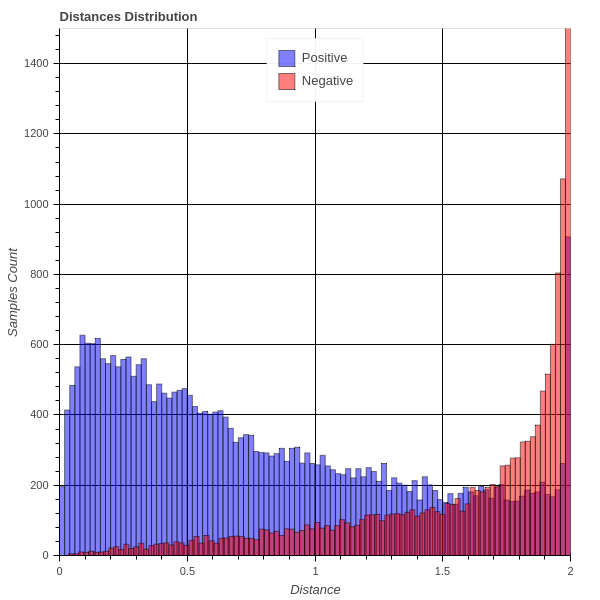
\includegraphics[scale=0.3]{histogram_reg.png}
        \caption{Distribution of the distances between feature vectors for the model using regular convolutions}
        \label{histogram_reg}
    \end{center}
\end{figure}

\begin{figure}
    \begin{center}
        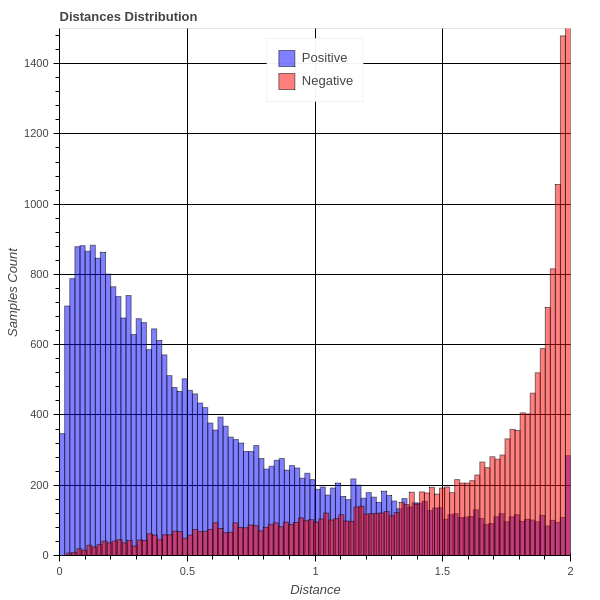
\includegraphics[scale=0.3]{histogram_sep.png}
        \caption{Distribution of the distances between feature vectors for the model using depthwise separable convolutions}
        \label{histogram_sep}
    \end{center}
\end{figure}

For tables \ref{triplet_regular_arch} and \ref{triplet_separable_arch}, all convolutional layers have a stride of 1x1 and are padded with zeros. For table \ref{triplet_regular_arch}, those layers also use the ReLU activation function. All max-pooling layers have a stride of 2x2 and a size of 2x2. All dense layers use the ReLU activation function. All dropout layers have a rate of 0.5. For table \ref{triplet_compare}, the inference time was calculated on 500 batches of 16 images, with processing limited to a single CPU core. For graphs \ref{histogram_reg} and \ref{histogram_sep}, the samples were extracted from 2000 batches of 16 image triples, and the y-axis was capped at 1500. The negative distribution exceeded this value by a very wide margin in its last bin.

Using the distributions shown in graphs \ref{histogram_reg} and \ref{histogram_sep}, a threshold was determined and a classifier created. It classifies 2 vectors with a distance between them greater or equal to the threshold as belonging to different people, otherwise belonging to the same person. The metrics for such classifier are shown in table \ref{triplet_class_compare}. The metrics in it were calculated on 2000 batches of 16 image pairs.

% Please add the following required packages to your document preamble:
% \usepackage{graphicx}
% \usepackage[table,xcdraw]{xcolor}
% If you use beamer only pass "xcolor=table" option, i.e. \documentclass[xcolor=table]{beamer}
\begin{table}[]
\centering
\caption{Metrics comparison between the classification models}
\label{triplet_class_compare}
\resizebox{\textwidth}{!}{%
\begin{tabular}{|c|c|c|c|c}
\cline{1-4}
\cellcolor[HTML]{9B9B9B}\textit{Convolution Type} &
  \cellcolor[HTML]{9B9B9B}\textit{Binary Accuracy} &
  \cellcolor[HTML]{9B9B9B}\textit{Precision} &
  \cellcolor[HTML]{9B9B9B}\textit{Recall} &
  \textit{} \\ \cline{1-4}
Regular   & 0.8441 & 0.847  & 0.8398 &                            \\ \cline{1-4}
Separable & 0.8576 & 0.8598 & 0.8546 &                            \\ \hline
\rowcolor[HTML]{9B9B9B} 
\textit{Convolution Type} &
  \textit{True Negatives} &
  \textit{False Positives} &
  \textit{False Negatives} &
  \multicolumn{1}{c|}{\cellcolor[HTML]{9B9B9B}\textit{True Positives}} \\ \hline
Regular   & 27145  & 4855   & 5125   & \multicolumn{1}{c|}{26875} \\ \hline
Separable & 27541  & 4459   & 4652   & \multicolumn{1}{c|}{27348} \\ \hline
\end{tabular}%
}
\end{table}



\section{Conclusions}

As seen in tables \ref{seg_compare}, \ref{triplet_compare} and \ref{triplet_class_compare}, depthwise separable convolutions provide a significant reduction in costs with a very low loss in metrics. For both bounding box detection and face verification, the models using depthwise separable convolutions are the ideal choice for real-world applications, due to their higher ratio of results to computational cost. 

It is evident however the benefits of including batch-normalization layers and activation functions without flat horizontal regions for those types of models. The several models that didn't converge at all on the segmentation aspect, compared to the fast conversion on the verification aspect show this. In that regard, the regular model on the verification step didn't include such layers, and would probably also benefit from including them. 

Also, on the verification step, the metrics were good, but not excellent. The triplet loss did generate a separable distribution between positive and negative pairs, but there is still a high overlap. Tables \ref{triplet_compare} and images \ref{histogram_reg} and \ref{histogram_sep} show that, while the negative class has tight distribution, the positive class has a much broader one, and this results in a higher false negatives count.

Other techniques would probably be able to improve the verification aspect. Techniques that could be attempted include:

\begin{itemize}
    \item Utilizing a bigger $\alpha$ (margin) for the triplet loss, which would make for a tighter positive distribution, since more distance would be needed for a pair to fall on the easy category.
    \item Pre-training the model on a face classification problem.
    \item Aligning the faces in the images through the use of detected landmarks, so that rotation and translation would become less relevant.
    \item For the comparison between 2 feature vectors, utilize a more complex classifier than a simple threshold on the distance between them.
\end{itemize}



\bibliographystyle{splncs04}
\bibliography{refs}

\end{document}
